\documentclass[fleqn]{article}
\usepackage[left=2cm,top=2cm,right=2cm,bottom=2cm]{geometry}
\usepackage{graphicx}
\usepackage{amsmath}
\usepackage{amssymb}
\usepackage{tikz}
\usetikzlibrary{}

\newcommand{\bigCI}{\mathrel{\text{\scalebox{1.07}{$\perp\mkern-10mu\perp$}}}}

\title{CS6730: Probabilistic Graphical Models \\ Homework-1}
\author{Arulkumar S (CS15D202)}
\date{\today}

\begin{document}
\maketitle
\section*{Solutions}
\subsection*{Q-1}

Consider a variant of the Monty hall problem, where the protocol is as follows. There are three doors, behind one of which is a car, and behind two of
which are goats. \textbf{You first choose a door. The host then randomly picks one of the two remaining doors.
It is observed to be a goat.} What is the probability that the car is behind the door you have already chosen? What would be a good Bayesian network
for modelling this problem?

\subsubsection*{answer:}

Let $F$ be the random variable to denote the first choice, $H$ be the random variable that denotes the choice of the host. Also, let $C (car), G
(goat)$ are the discrete states of random variables $F \& H$.

\begin{eqnarray}
\begin{aligned}
P(F=C | H=G) &= \frac{P(F=C, H=G)}{P(H=G)}\\
			 &= \frac{P(F=C)P(H=G|F=C)}{\sum_{i=\{G,C\}} P(F=i, H=G)}\\ 
			 &= \frac{\frac{1}{3} * 1}{P(F=C)P(H=G|F=C) + P(F=G)P(H=G|F=G)}\\
			 &= \frac{\frac{1}{3} * 1}{(\frac{1}{3} * 1) + (\frac{2}{3} * \frac{1}{2})}\\
			 &= \frac{1}{2}
\end{aligned}
\end{eqnarray}

\noindent\rule{\textwidth}{1pt}

\subsection*{Q-2}
\subsubsection*{answer:}

\subsubsection*{Conditional independencies for Graphs}
(I) $C \bigCI D | A, B$\\
\hspace*{1em} $A \bigCI B$\\\\
(II) $A \bigCI B, D$\\
\hspace*{1em} $C \bigCI B, D$\\\\
(III) $A \bigCI B, C, D$\\
\hspace*{1em} $B \bigCI C, D$\\
\hspace*{1em} $C \bigCI D$\\

\subsubsection*{Conditional independencies for Tables}

(I)
{
\small $P(A=0) = 0.5, P(A=1) = 0.5, $\\
\hspace*{1em} $P(B=0) = 0.5, P(B=1) = 0.5$\\
\hspace*{1em} $P(C=0) = 0.5, P(C=1) = 0.5$\\
\hspace*{1em} $P(D=0) = 0.5, P(D=1) = 0.5$\\
\hspace*{1em} $P(A=0, B=0) = 0.5, P(A=0, B=1) = 0, P(A=1, B=0) = 0, P(A=1, B=1) = 0.5$\\
\hspace*{1em} $P(A=0, C=0) = 0.5, P(A=0, C=1) = 0, P(A=1, C=0) = 0, P(A=1, C=1) = 0.5$\\
\hspace*{1em} $P(A=0, D=0) = 0.5, P(A=0, D=1) = 0, P(A=1, D=0) = 0, P(A=1, D=1) = 0.5$\\
\hspace*{1em} $P(B=0, C=0) = 0.5, P(B=0, C=1) = 0, P(B=1, C=0) = 0, P(B=1, C=1) = 0.5$\\
\hspace*{1em} $P(B=0, D=0) = 0.5, P(B=0, D=1) = 0, P(B=1, D=0) = 0, P(B=1, D=1) = 0.5$\\
\hspace*{1em} $P(C=0, D=0) = 0.5, P(C=0, D=1) = 0, P(C=1, D=0) = 0, P(C=1, D=1) = 0.5$\\
}

Conditional independencies:

\begin{itemize}
  \item From the table as well as the probabilities calculated above, we can notice that the probability is non-zero when A,B,C,D = (0,0,0,0) or
  (1,1,1,1). So, itseems that all the random variables are depending on one particular random variable. But we could not find out which variable
  it is. So, No conclusion about conditional independencies can be made.
\end{itemize}


\noindent(II)
{
\small
 $P(A=0) = 0.5, P(A=1) = 0.5, $\\
\hspace*{1em} $P(B=0) = 0.5, P(B=1) = 0.5$\\
\hspace*{1em} $P(C=0) = 0.5, P(C=1) = 0.5$\\
\hspace*{1em} $P(D=0) = 0.6, P(D=1) = 0.4$\\
\hspace*{1em} $P(A=0, B=0) = 0.25, P(A=0, B=1) = 0.25, P(A=1, B=0) = 0.25, P(A=1, B=1) = 0.25$\\
\hspace*{1em} $P(A=0, C=0) = 0.15, P(A=0, C=1) = 0.35, P(A=1, C=0) = 0.25, P(A=1, C=1) = 0.25$\\
\hspace*{1em} $P(A=0, D=0) = 0.20, P(A=0, D=1) = 0.30, P(A=1, D=0) = 0.40, P(A=1, D=1) = 0.10$\\
\hspace*{1em} $P(B=0, C=0) = 0.20, P(B=0, C=1) = 0.30, P(B=1, C=0) = 0.30, P(B=1, C=1) = 0.20$\\
\hspace*{1em} $P(B=0, D=0) = 0.25, P(B=0, D=1) = 0.25, P(B=1, D=0) = 0.25, P(B=1, D=1) = 0.25$\\
\hspace*{1em} $P(C=0, D=0) = 0.35, P(C=0, D=1) = 0.15, P(C=1, D=0) = 0.25, P(C=1, D=1) = 0.25$\\
}

Conditional independencies:

\begin{itemize}
  \item $A \bigCI B$
  \item $C \bigCI D | A, B$ 
  
  \begin{eqnarray*}
  \begin{aligned}
  P(C=0, D=0 | A=0,B=0)&=\frac{P(A=0,B=0,C=0,D=0)}{P(A=0,B=0)}=\frac{0.015}{0.25}=\frac{3}{50}\\ 
  &= P(C=0|A=0,B=0).P(D=0|A=0,B=0)\\
  &=\frac{\sum_D P(A=0,B=0,C=0,D). \sum_C P(A=0,B=0,C,D=0)}{P(A=0,B=0)*P(A=0,B=0)}\\
  &=\frac{0.05*0.075}{0.25 * 0.25}=\frac{3}{50},
  \end{aligned}
  \end{eqnarray*}
   and so on
\end{itemize}

\noindent(III)
{
\small
 $P(A=0) = 1, P(A=1) = 0, $\\
\hspace*{1em} $P(B=0) = 0.25, P(B=1) = 0.75$\\
\hspace*{1em} $P(C=0) = 0.20, P(C=1) = 0.80$\\
\hspace*{1em} $P(D=0) = 0.40, P(D=1) = 0.60$\\
\hspace*{1em} $P(A=0, B=0) = 0.25, P(A=0, B=1) = 0.75, P(A=1, B=0) = 0, P(A=1, B=1) = 0$\\
\hspace*{1em} $P(A=0, C=0) = 0.20, P(A=0, C=1) = 0.80, P(A=1, C=0) = 0, P(A=1, C=1) = 0$\\
\hspace*{1em} $P(A=0, D=0) = 0.40, P(A=0, D=1) = 0.60, P(A=1, D=0) = 0, P(A=1, D=1) = 0$\\
\hspace*{1em} $P(B=0, C=0) = 0.05, P(B=0, C=1) = 0.20, P(B=1, C=0) = 0.15, P(B=1, C=1) = 0.60$\\
\hspace*{1em} $P(B=0, D=0) = 0.10, P(B=0, D=1) = 0.15, P(B=1, D=0) = 0.30, P(B=1, D=1) = 0.45$\\
\hspace*{1em} $P(C=0, D=0) = 0.08, P(C=0, D=1) = 0.12, P(C=1, D=0) = 0.32, P(C=1, D=1) = 0.48$\\
}

Conditional independencies:

\begin{itemize}
  \item $A \bigCI B, C, D$ (i.e., $P(A=i, B=j) = P(A=i).P(B=j)$ and so on)
  \item $B \bigCI C, D$
  \item $C \bigCI D$
\end{itemize}

\subsection*{Graphs vs. Table distributions}
\begin{itemize}
  \item Distribution (I) is not conforming with any of the graphs given
  \item Distribution (II) is conforming with the graph (I)
  \item Distribution (III) is conforming with graph (III)
\end{itemize}

\noindent\rule{\textwidth}{1pt}

\subsection*{Q-3}
\subsubsection*{answer:}

\subsection*{Distribution tables:}
(a)
\begin{center}
\begin{tabular}{ c c c c c }
                & \text{C=0,D=0} & \text{C=0,D=1} & \text{C=1,D=0} & \text{C=1,D=1} \\ 
 \text{A=0,B=0} & 0 & 0 &0 &0 \\  
 \text{A=0,B=1} & 0 & 0.5 & 0.5 & 0\\  
 \text{A=1,B=0} & 0 & 0 & 0 & 0 \\  
 \text{A=1,B=1} & 0 & 0 & 0 & 0     
\end{tabular}
\end{center}

(b)
\begin{center}
\begin{tabular}{ c c c c c }
                & \text{C=0,D=0} & \text{C=0,D=1} & \text{C=1,D=0} & \text{C=1,D=1} \\ 
 \text{A=0,B=0} & 0.25 & 0 & 0 & 0 \\  
 \text{A=0,B=1} & 0 & 0.25 & 0 & 0 \\  
 \text{A=1,B=0} & 0 & 0 & 0.25 & 0 \\  
 \text{A=1,B=1} & 0 & 0 & 0 & 0.25     
\end{tabular}
\end{center}

(c) $(A \bigCI C | B, D), (B \bigCI D | A, C)$ - Not possible to be represented by Bayesian network

\subsection*{Bayesian networks:}

\begin{figure}[!ht]
\centering
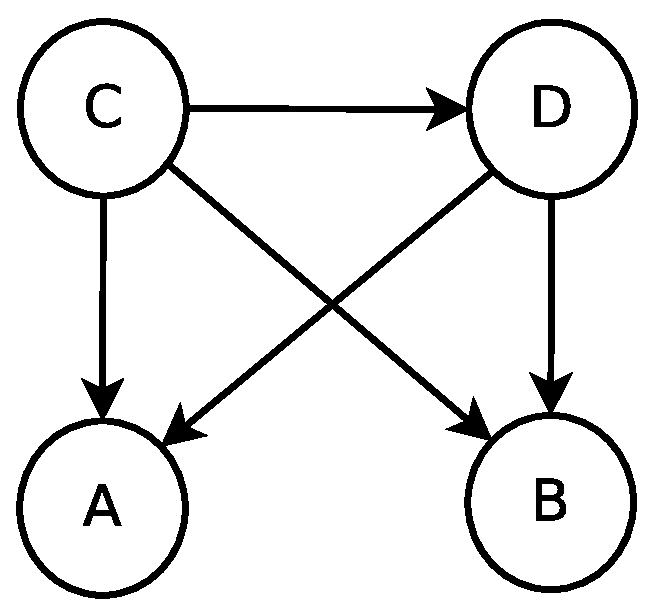
\includegraphics[scale=0.3]{./HW1_diagrams_3a}
\caption{(a) $A \bigCI B | C, D$}
\end{figure}

\begin{figure}[!ht]
\centering
\includegraphics[scale=0.3]{./HW1_diagrams_3b}
\caption{(b)(A \bigCI B | C, D), (C \bigCI D) }
\end{figure}

(c) $(A \bigCI C | B, D), (B \bigCI D | A, C)$ - Not possible to be represented by Bayesian network, as it introduces cycle in the network


\noindent\rule{\textwidth}{1pt}
\subsection*{Q-4}

Consider the Bayesian network given below:

Consider a distribution over 8 random variables $X_1, X_2, \dots, X_8$ given by the Bayesian network to the left.

\begin{enumerate}
  \item Give the largest set of random variables that is independent of $X_3$. 
  \subsubsection*{answer:} $X_3 \bigCI X_2, X_5, X_7$
  \item Give the largest set of random variables that is independent of $X_3$, conditioned on $X_1$.
  \subsubsection*{answer:} $X_3 \bigCI X_2, X_4, X_5, X_7, X_8 | X_4$
  \item Give the largest set of random variables that is independent of $X_3$, conditioned on $X_1$ and $X_4$.
  \subsubsection*{answer:} $X_3 \bigCI X_2, X_4, X_5, X_7, X_8 | X_1, X_4$
\end{enumerate}

\noindent\rule{\textwidth}{1pt}




\end{document}